\documentclass[tikz,border=8pt]{standalone}
\usepackage{amsmath}
\usetikzlibrary{arrows.meta,positioning,fit}

\begin{document}
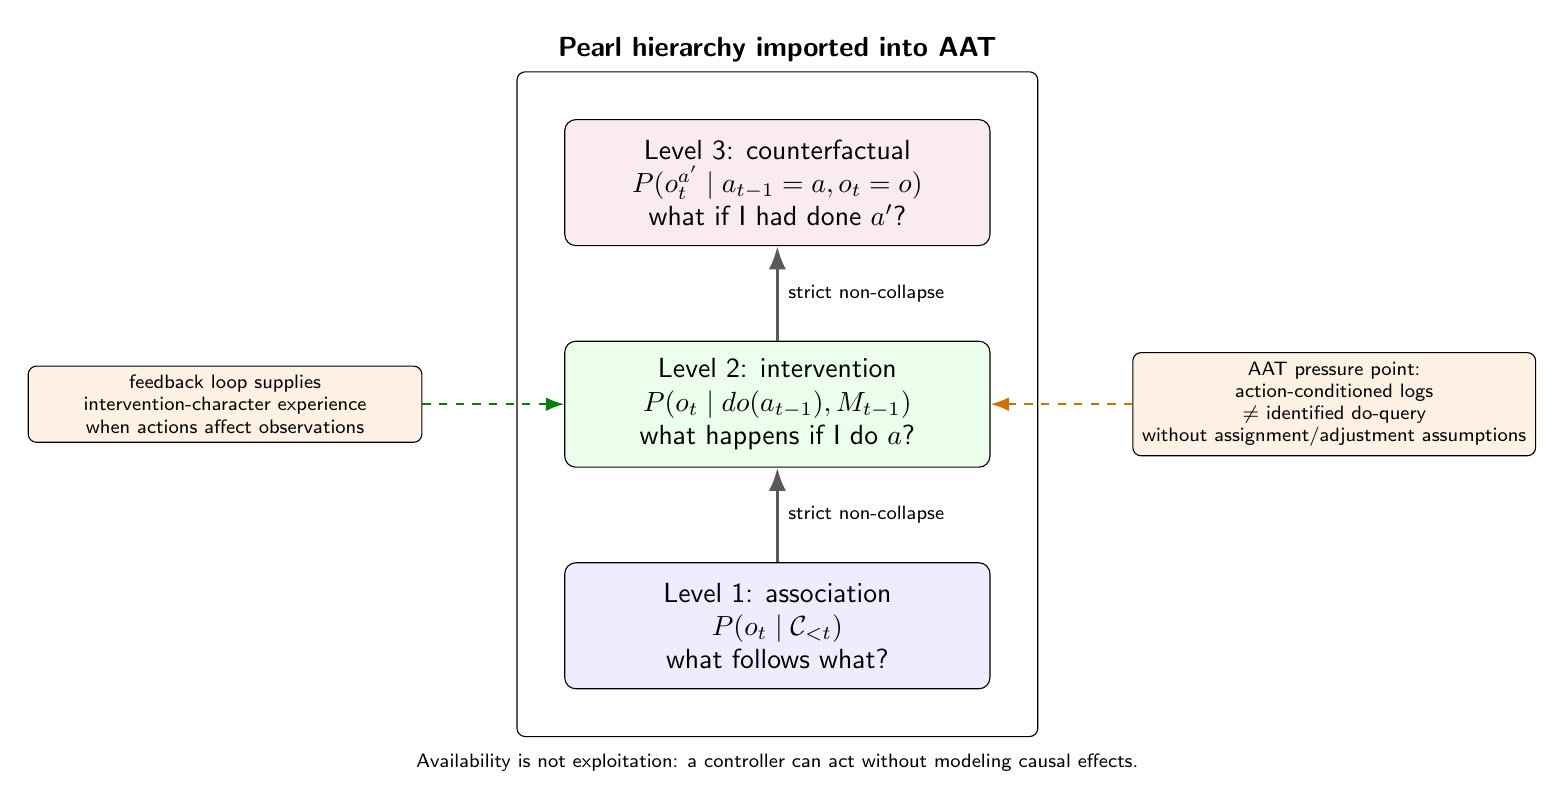
\begin{tikzpicture}[
  font=\sffamily,
  level/.style={draw, rounded corners=4pt, align=center, minimum width=54mm, minimum height=16mm, fill=white},
  arrow/.style={-Latex, very thick, draw=black!65},
  warn/.style={draw, rounded corners=3pt, align=center, fill=orange!10, font=\sffamily\scriptsize, minimum width=50mm},
  note/.style={align=center, font=\sffamily\scriptsize}
]

\node[level, fill=blue!7] (l1) {Level 1: association\\$P(o_t\mid \mathcal{C}_{<t})$\\what follows what?};
\node[level, above=12mm of l1, fill=green!8] (l2) {Level 2: intervention\\$P(o_t\mid do(a_{t-1}),M_{t-1})$\\what happens if I do $a$?};
\node[level, above=12mm of l2, fill=purple!8] (l3) {Level 3: counterfactual\\$P(o_t^{a'}\mid a_{t-1}=a,o_t=o)$\\what if I had done $a'$?};

\draw[arrow] (l1) -- node[right, note] {strict non-collapse} (l2);
\draw[arrow] (l2) -- node[right, note] {strict non-collapse} (l3);

\node[warn, right=18mm of l2] (caveat)
  {AAT pressure point:\\action-conditioned logs\\$\neq$ identified do-query\\without assignment/adjustment assumptions};
\draw[-Latex, thick, dashed, draw=orange!85!black] (caveat) -- (l2);

\node[warn, left=18mm of l2] (loop)
  {feedback loop supplies\\intervention-character experience\\when actions affect observations};
\draw[-Latex, thick, dashed, draw=green!50!black] (loop) -- (l2);

\node[note, below=7mm of l1] {Availability is not exploitation: a controller can act without modeling causal effects.};

\node[draw, rounded corners=3pt, fit=(l1)(l2)(l3), inner sep=6mm,
  label={[font=\sffamily\bfseries]above:Pearl hierarchy imported into AAT}] {};

\end{tikzpicture}
\end{document}
